\documentclass[journal]{vgtc}                % final (journal style)

%% These few lines make a distinction between latex and pdflatex calls and they
%% bring in essential packages for graphics and font handling.
%% Note that due to the \DeclareGraphicsExtensions{} call it is no longer necessary
%% to provide the the path and extension of a graphics file:
%% 
\includegraphics{diamondrule} is completely sufficient.
%%
\ifpdf%                                % if we use pdflatex
  \pdfoutput=1\relax                   % create PDFs from pdfLaTeX
  \pdfcompresslevel=9                  % PDF Compression
  \pdfoptionpdfminorversion=7          % create PDF 1.7
  \ExecuteOptions{pdftex}
  \usepackage{graphicx}                % allow us to embed graphics files
  \DeclareGraphicsExtensions{.pdf,.png,.jpg,.jpeg} % for pdflatex we expect .pdf, .png, or .jpg files
\else%                                 % else we use pure latex
  \ExecuteOptions{dvips}
  \usepackage{graphicx}                % allow us to embed graphics files
  \DeclareGraphicsExtensions{.eps}     % for pure latex we expect eps files
\fi%

%% it is recomended to use ``\autoref{sec:bla}'' instead of ``Fig.~\ref{sec:bla}''
\graphicspath{ {pictures/} } % where to search for the images

\usepackage{microtype}                 % use micro-typography (slightly more compact, better to read)
\usepackage{hyperref}
\usepackage{listings}
\lstset{language=SQL,caption={The file nba.sql that implements our ER Diagrams.}}

\PassOptionsToPackage{warn}{textcomp}  % to address font issues with \textrightarrow
\usepackage{times}                     % we use Times as the main font
\renewcommand*\ttdefault{txtt}         % a nicer typewriter font

%% declare the category of your paper, only shown in review mode
\vgtccategory{Research}

\title{Visualizations of How NBA Player Salaries Relate to Individual and Team Performance}

\author{Alex Hoffer, Austin Nguyen, Prathveer Rai}

\renewcommand{\manuscriptnotetxt}{}

\vgtcinsertpkg

\begin{document}

\maketitle

\section{Introduction}
The following subsections explain what the problem is we hope to elucidate through the use of information visualization, the importance of visualization as a tool in understanding the problem, potential users of our visualizations, and how we plan on approaching our visualizations in subsequent assignments.

\subsection{Problem Explanation}
In the National Basketball Association (NBA), teams are allowed 15 players on their rosters and each player is paid a salary established in their contract. According to Wikipedia, each team can spend a total of \$102 million on their players, and this is referred to as their \emph{salary cap}. The salary which a player is given can be based on a number of complex factors such as an impending increase in salary cap, a demand for that player's skill set, or improvements to team chemistry, but it can generally be agreed that the amount a player is paid should correspond to their on-court performance. It is therefore an advantage for teams to get good players on cheap contracts so that they can have flexibility within the salary cap to spend money on getting more good players. An excellent example of a great player on a cheap contract is Stephen Curry, who signed a meager contract when he was injurious, and since then has improved to become a premier NBA player. On the flip side, since there is a salary cap, teams should be wary of spending a lot of money on players who do not deserve it. Some examples of players who are generally agreed to be overpaid considering their skill level are Timofey Mozgov of the Los Angeles Lakers and Bismack Biyombo of the Orlando Magic. The problem, then, is that since each team must carefully spend their money in order to maximize team success, some players end up overpaid, and this leads to teams underperforming. But what aspects of player performance can be used to assess whether or not they deserve their salary? It is the goal of this project to discover through the use of information visualization how statistical domains of player performance such as points per game, team performance in terms of their win/loss record, and player salary are related in an effort to inform teams on which players are actually worth their price tag so they may more wisely allocate their financial resources and thus improve their chances of winning.  

\subsection{Importance of Visualization}
It is easy to get lost amidst the plethora of statistics there are available to fans of the NBA. From simple statistics like points or assists per game to complex measurements such as Player Efficiency Rating (PER), those interested in evaluating a player may not get an accurate impression because of how difficult and unclear it is to read these numbers and mentally compile them in a meaningful way. Here is where visualization comes in: being able to graphically represent basketball statistics means that we can tell a story about a player's performance in relation to his salary without bogging the reader down with unnecessary details. We can facilitate their understanding by presenting the information they desire to know in a way that makes more sense to them than merely showing them a table of numbers.  

\subsection{Potential Users and User Groups}
There are a myriad of potential users of the information visualizations we propose. A sample of groups that may be interested are listed below:
\begin{itemize}
\item \emph{NBA Fans: } Fans of the NBA may want to see how the players on the team they like are contributing to their team's success or are, in fact, detrimental.
\item \emph{NBA Management: } Those who occupy management positions that are in charge of player personnel within NBA teams want to know how much money they should offer a player, and knowing how much bang for their buck they've gotten from a player will aid in this pursuit.
\item \emph{NBA Agents: } Agents of NBA players will want to know how much money they should demand for their player in the course of contract negotiation.
\end{itemize}

\subsection{General Approach to Visualization}
Our approach to visualization will be inspired by the interface provided when making in-game substitutions in the video game \emph{FIFA 17} as well as the following image provided by Rami Moghadam at \url{http://ramimo.com/2013-NBA-All-Stars}. In his image, he has players from the NBA All-Star Game represented as circular graphs consisting of slices such as \emph{Fouls} and \emph{Minutes} with cells that begin at 0 and increase incrementally to large numbers. There is coloration within each slice that reaches up to the cell that corresponds to their season average as of the All-Star Game. When we look at the graph, we can easily see things like how many minutes they've played and how much they've scored given those minutes. We want to use this circular graph with slices, cells, and methodological coloration. Our slices, like Moghadam's, will correspond to statistical categories we find interesting, and the values in our cells will increment in the same fashion, but we will also have slices devoted to \textbf{team wins and losses} as well as \textbf{paid salary}, among other possible categories. Naturally, we will have to experiment with different statistical categories to see which ones we think are useful. We believe this approach to visualization will help easily create a narrative about whether a player's performance warrants their price tag.

\section{Visualization Tasks}
The questions we hope to address with the visualization are as follows:
\begin{itemize}
\item What statistical categories are useful to look at when considering whether a player is worth what he's paid?
\item Given those stats, is a certain player overpaid?
\item Given those stats, is a certain player underpaid?
\end{itemize}

We want to ask these questions about all players, but ultimately our project should consist only of visualizations where a player is overpaid or underpaid, for these are the players who have the most interesting narratives to consider.

\section{Data Sources}
Luckily, all statistics that relate to NBA players and teams as well as pay information are conveniently available on the ESPN website. Specificially, the data we will use can be found here: \url{http://stats.nba.com/players/traditional/}. Since these are just raw statistics not subject to bias, one source is enough for our purposes.

\section{Data Organization in Terms of ER Diagram}
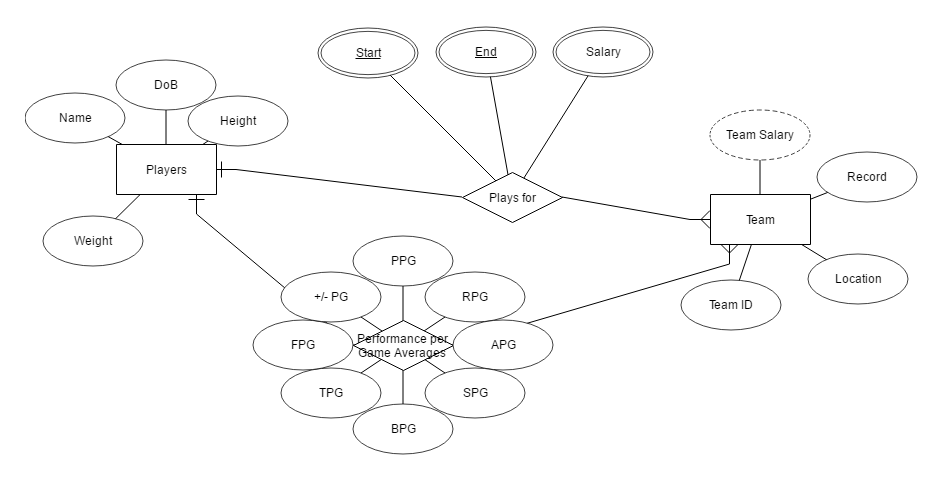
\includegraphics[width=9cm, height=9cm]{ERdiagram}

\section{Relational Database Implementation of ER Diagrams}
\emph{Listing 1} is the code we have written to implement our ER Diagrams in the form of relational databases:
\begin{lstlisting}
SET SQL_MODE = "NO_AUTO_VALUE_ON_ZERO";
SET time_zone = "+00:00";


/*!40101 SET @OLD_CHARACTER_SET_CLIENT=
@@CHARACTER_SET_CLIENT */;
/*!40101 SET @OLD_CHARACTER_SET_RESULTS=
@@CHARACTER_SET_RESULTS */;
/*!40101 SET @OLD_COLLATION_CONNECTION=
@@COLLATION_CONNECTION */;
/*!40101 SET NAMES utf8mb4 */;

--
-- Database: `nba`
--

--
--
-- Table structure for table `performance`
--

CREATE TABLE `performance` (
  `id` int(11) NOT NULL,
  `PPG` int(11) NOT NULL,
  `RPG` int(11) NOT NULL,
  `BPG` int(11) NOT NULL,
  `APG` int(11) NOT NULL,
  `SPG` int(11) NOT NULL,
  `TPG` int(11) NOT NULL,
  `PG` int(11) NOT NULL,
  `FPG` int(11) NOT NULL
) ENGINE=InnoDB DEFAULT CHARSET=latin1;

--
-- Table structure for table `players`
--

CREATE TABLE `players` (
  `id` int(11) NOT NULL,
  `Name` text NOT NULL,
  `Height` int(11) NOT NULL,
  `Weight` int(11) NOT NULL
) ENGINE=InnoDB DEFAULT CHARSET=latin1;

--
-- Table structure for table `player_salary`
--

CREATE TABLE `player_salary` (
  `id` int(11) NOT NULL,
  `Start_date` int(11) NOT NULL,
  `End_date` int(11) NOT NULL,
  `Salary` int(11) NOT NULL
) ENGINE=InnoDB DEFAULT CHARSET=latin1;

--
-- Table structure for table `team`
--

CREATE TABLE `team` (
  `id` int(11) NOT NULL,
  `Location` mediumtext NOT NULL,
  `Record` int(11) NOT NULL,
  `Player_sal_id` int(11) NOT NULL,
  `performance` int(11) NOT NULL
) ENGINE=InnoDB DEFAULT CHARSET=latin1;

--
-- Indexes for dumped tables
--

--
-- Indexes for table `performance`
--
ALTER TABLE `performance`
  ADD PRIMARY KEY (`id`);

--
-- Indexes for table `players`
--
ALTER TABLE `players`
  ADD PRIMARY KEY (`id`);

--
-- Indexes for table `player_salary`
--
ALTER TABLE `player_salary`
  ADD PRIMARY KEY (`id`);

--
-- Indexes for table `team`
--
ALTER TABLE `team`
  ADD PRIMARY KEY (`id`),
  ADD UNIQUE KEY `Player_sal_id` (`Player_sal_id`),
  ADD UNIQUE KEY `performance` (`performance`);

--
-- AUTO_INCREMENT for dumped tables
--

--
-- AUTO_INCREMENT for table `players`
--
ALTER TABLE `players`
  MODIFY `id` int(11) NOT NULL AUTO_INCREMENT;
--
-- AUTO_INCREMENT for table `player_salary`
--
ALTER TABLE `player_salary`
  MODIFY `id` int(11) NOT NULL AUTO_INCREMENT;
--
-- AUTO_INCREMENT for table `team`
--
ALTER TABLE `team`
  MODIFY `id` int(11) NOT NULL AUTO_INCREMENT;
/*!40101 SET CHARACTER_SET_CLIENT=
@OLD_CHARACTER_SET_CLIENT */;
/*!40101 SET CHARACTER_SET_RESULTS=
@OLD_CHARACTER_SET_RESULTS */;
/*!40101 SET COLLATION_CONNECTION=
@OLD_COLLATION_CONNECTION */;

\end{lstlisting}

\section{Design of the Visualization Interface}
The design interface follows the visualization idea explained earlier. We essentially create a circular statistical graph. The graph is split into separate categories which represent the performance factors. And based on this visualized data, end users can identify whether the player’s performance justifies his salary. Perhaps the end user could interact with a module where they can select from a set of players we find interesting to look at and maybe be able to select from a set of stats we find interesting as well.
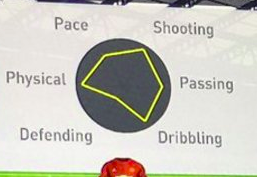
\includegraphics[width=9cm, height=9cm]{stats}

\bibliographystyle{abbrv-doi}
\bibliography{template}

\end{document}

